\FloatBarrier      % resolve any leftover floats from the two-column body
\clearpage         % force them onto their own page, cleanly
\onecolumn         % now switch — nothing pending to flush
\appendix

\section{Full Regression Tables}
\label{app:regression_tables}

This appendix provides the complete statistical results from the linear mixed-effects 
regression model used to quantify the performance impact of each query chokepoint. 

Table~\ref{tab:full_cache_hit_rate} presents the fixed effects ($\boldsymbol{\beta}$) 
of chokepoint additions (+) and removals (-) on the cache hit rate.

% Require \usepackage{booktabs} in preamble
\begin{table}[H]
\caption{Fixed effects and goodness-of-fit for cache hit rate. Standard errors in parentheses.}
\label{tab:full_cache_hit_rate}
\begin{tabular}{lccc}
\toprule
 & S & M & L \\
\midrule
$Y_{i,t-1}$ & -1.007*** (0.025) & -0.982*** (0.024) & -0.949*** (0.024) \\
P-1+ & 0.146*** (0.035) & 0.152*** (0.035) & 0.075* (0.035) \\
P-1- & 0.024 (0.053) & 0.080 (0.054) & 0.089 (0.054) \\
P-2+ & 0.089* (0.043) & 0.067 (0.043) & 0.050 (0.043) \\
P-2- & 0.240*** (0.050) & 0.230*** (0.051) & 0.111* (0.051) \\
P-3+ & -0.041 (0.035) & 0.012 (0.035) & 0.052 (0.035) \\
P-3- & 0.210*** (0.049) & 0.103* (0.050) & 0.117* (0.050) \\
P-4+ & -0.141*** (0.032) & -0.107*** (0.032) & -0.086** (0.032) \\
P-4- & 0.210*** (0.044) & 0.223*** (0.044) & 0.214*** (0.044) \\
T-1+ & 0.287*** (0.051) & 0.257*** (0.052) & 0.225*** (0.052) \\
T-1- & -0.151* (0.067) & 0.052 (0.068) & 0.025 (0.068) \\
T-2+ & -0.382*** (0.029) & -0.385*** (0.029) & -0.361*** (0.029) \\
T-2- & 0.343*** (0.037) & 0.368*** (0.037) & 0.376*** (0.037) \\
T-3+ & -0.135* (0.057) & -0.174** (0.058) & -0.114 (0.058) \\
T-3- & -0.155* (0.070) & -0.300*** (0.071) & -0.160* (0.071) \\
T-4+ & 0.068 (0.057) & 0.043 (0.058) & 0.072 (0.057) \\
T-4- & -0.006 (0.068) & 0.010 (0.068) & 0.035 (0.068) \\
\midrule
Log-Likelihood & -362.336 & -379.669 & -378.989 \\
Marginal $R^2$ & 0.284 & 0.234 & 0.222 \\
Conditional $R^2$ & 0.913 & 0.922 & 0.920 \\
ICC & 0.878 & 0.898 & 0.897 \\
\bottomrule
\end{tabular}
\end{table}

\FloatBarrier

Table~\ref{tab:full_discovered_sources} lists the isolated structural impacts and fixed effects for Discovered Sources.

\begin{table}[H]
\caption{Fixed effects and goodness-of-fit for cache hit rate. Standard errors in parentheses.}
\label{tab:full_discovered_sources}
\begin{tabular}{lccc}
\toprule
 & S & M & L \\
\midrule
$Y_{i,t-1}$ & -0.099 (0.058) & -0.170** (0.065) & -0.162* (0.072) \\
P-1+ & -0.485 (0.481) & -0.916 (0.524) & -0.971 (0.524) \\
P-1- & -1.354 (0.943) & -1.228 (0.947) & 0.442 (0.914) \\
P-2+ & 0.253 (0.534) & 0.097 (0.577) & 0.456 (0.598) \\
P-2- & -0.414 (0.801) & 0.545 (0.829) & -0.938 (0.816) \\
P-3+ & 0.427 (0.441) & 0.430 (0.477) & 0.510 (0.492) \\
P-3- & -2.592*** (0.635) & -2.026** (0.685) & -2.759*** (0.709) \\
P-4+ & 2.036*** (0.446) & 2.012*** (0.473) & 2.366*** (0.480) \\
P-4- & -4.095*** (0.666) & -2.981*** (0.695) & -4.120*** (0.693) \\
T-1+ & 1.203 (0.623) & 0.549 (0.676) & 0.336 (0.706) \\
T-1- & -0.156 (0.964) & -0.617 (1.021) & -0.319 (1.026) \\
T-2+ & 0.144 (0.393) & 0.335 (0.420) & 0.415 (0.428) \\
T-2- & -1.231* (0.598) & -1.453* (0.613) & -1.761** (0.602) \\
T-3+ & -0.119 (0.707) & 0.813 (0.765) & -0.074 (0.802) \\
T-3- & -1.979 (1.066) & -2.306* (1.111) & -1.214 (1.107) \\
T-4+ & -0.588 (0.687) & -1.032 (0.751) & -1.109 (0.784) \\
T-4- & 2.302* (1.068) & 2.134 (1.100) & 2.289* (1.088) \\
\midrule
Log-Likelihood & -4048.816 & -4046.863 & -4000.735 \\
Marginal $R^2$ & 0.155 & 0.129 & 0.152 \\
Conditional $R^2$ & 0.214 & 0.240 & 0.329 \\
ICC & 0.070 & 0.127 & 0.209 \\
\bottomrule
\end{tabular}
\end{table}


Table~\ref{tab:full_execution_time} outlines the fixed effects for the Execution Time metric.

% Require \usepackage{booktabs} in preamble
\begin{table}[hbt!]
\caption{Fixed effects and goodness-of-fit for execution time. Standard errors in parentheses.}
\label{tab:full_execution_time}
\begin{tabular}{lccc}
\toprule
 & S & M & L \\
\midrule
$Y_{i,t-1}$  & -0.810*** (0.111) & -0.698*** (0.085) & -0.669*** (0.084) \\
P-1+ & 0.791 (0.716) & 0.640 (0.717) & 0.605 (0.730) \\
P-1- & -4.737*** (1.174) & -2.139 (1.214) & -1.723 (1.245) \\
P-2+ & -1.174 (0.851) & -0.330 (0.842) & -0.087 (0.854) \\
P-2- & 4.990*** (1.082) & 4.619*** (1.106) & 2.781* (1.130) \\
P-3+ & 1.245 (0.695) & 1.331 (0.689) & 1.973** (0.700) \\
P-3- & 3.252** (1.030) & 1.040 (1.002) & 1.443 (1.026) \\
P-4+ & 5.233*** (0.671) & 3.918*** (0.667) & 4.069*** (0.682) \\
P-4- & -5.515*** (0.933) & -4.930*** (0.944) & -4.452*** (0.966) \\
T-1+ & -1.850 (1.037) & -0.255 (1.007) & 0.002 (1.011) \\
T-1- & -5.762*** (1.461) & -4.566** (1.450) & -5.415*** (1.497) \\
T-2+ & 1.926*** (0.582) & 1.376* (0.581) & 1.501* (0.593) \\
T-2- & -1.991* (0.791) & -1.411 (0.811) & -1.196 (0.830) \\
T-3+ & 4.974*** (1.152) & 3.868*** (1.130) & 3.243** (1.137) \\
T-3- & 2.930 (1.523) & 1.522 (1.528) & 3.375* (1.571) \\
T-4+ & 1.104 (1.141) & 0.561 (1.132) & 0.352 (1.149) \\
T-4- & -3.122* (1.474) & -1.642 (1.495) & -1.542 (1.539) \\
\midrule
Log-Likelihood & -4345.931 & -4381.203 & -4413.325 \\
Marginal $R^2$ & 0.247 & 0.209 & 0.202 \\
Conditional $R^2$ & 0.556 & 0.455 & 0.432 \\
ICC & 0.411 & 0.311 & 0.288 \\
\bottomrule
\end{tabular}
\end{table}
\newpage
\section{Full Synthetic Hit Rate Figures}
\label{app:synth-hitrate}
This section provides the full results of the synthetic hit rate experiments summarized in Section~\ref{sec:evaluation}. 
Figures~\ref{fig:full-theoretical-unindexed},~\ref{fig:full-theoretical-indexed},~\ref{fig:full-theoretical-store}, 
and~\ref{fig:full-theoretical-disk}
show the results for the LRU-based unindexed cache, LRU-based indexed cache, the in-memory store cache, and the disk-based store cache, respectively.

\begin{figure*}[!h]
    \centering
    % Ensure the filename matches your generated PDF
    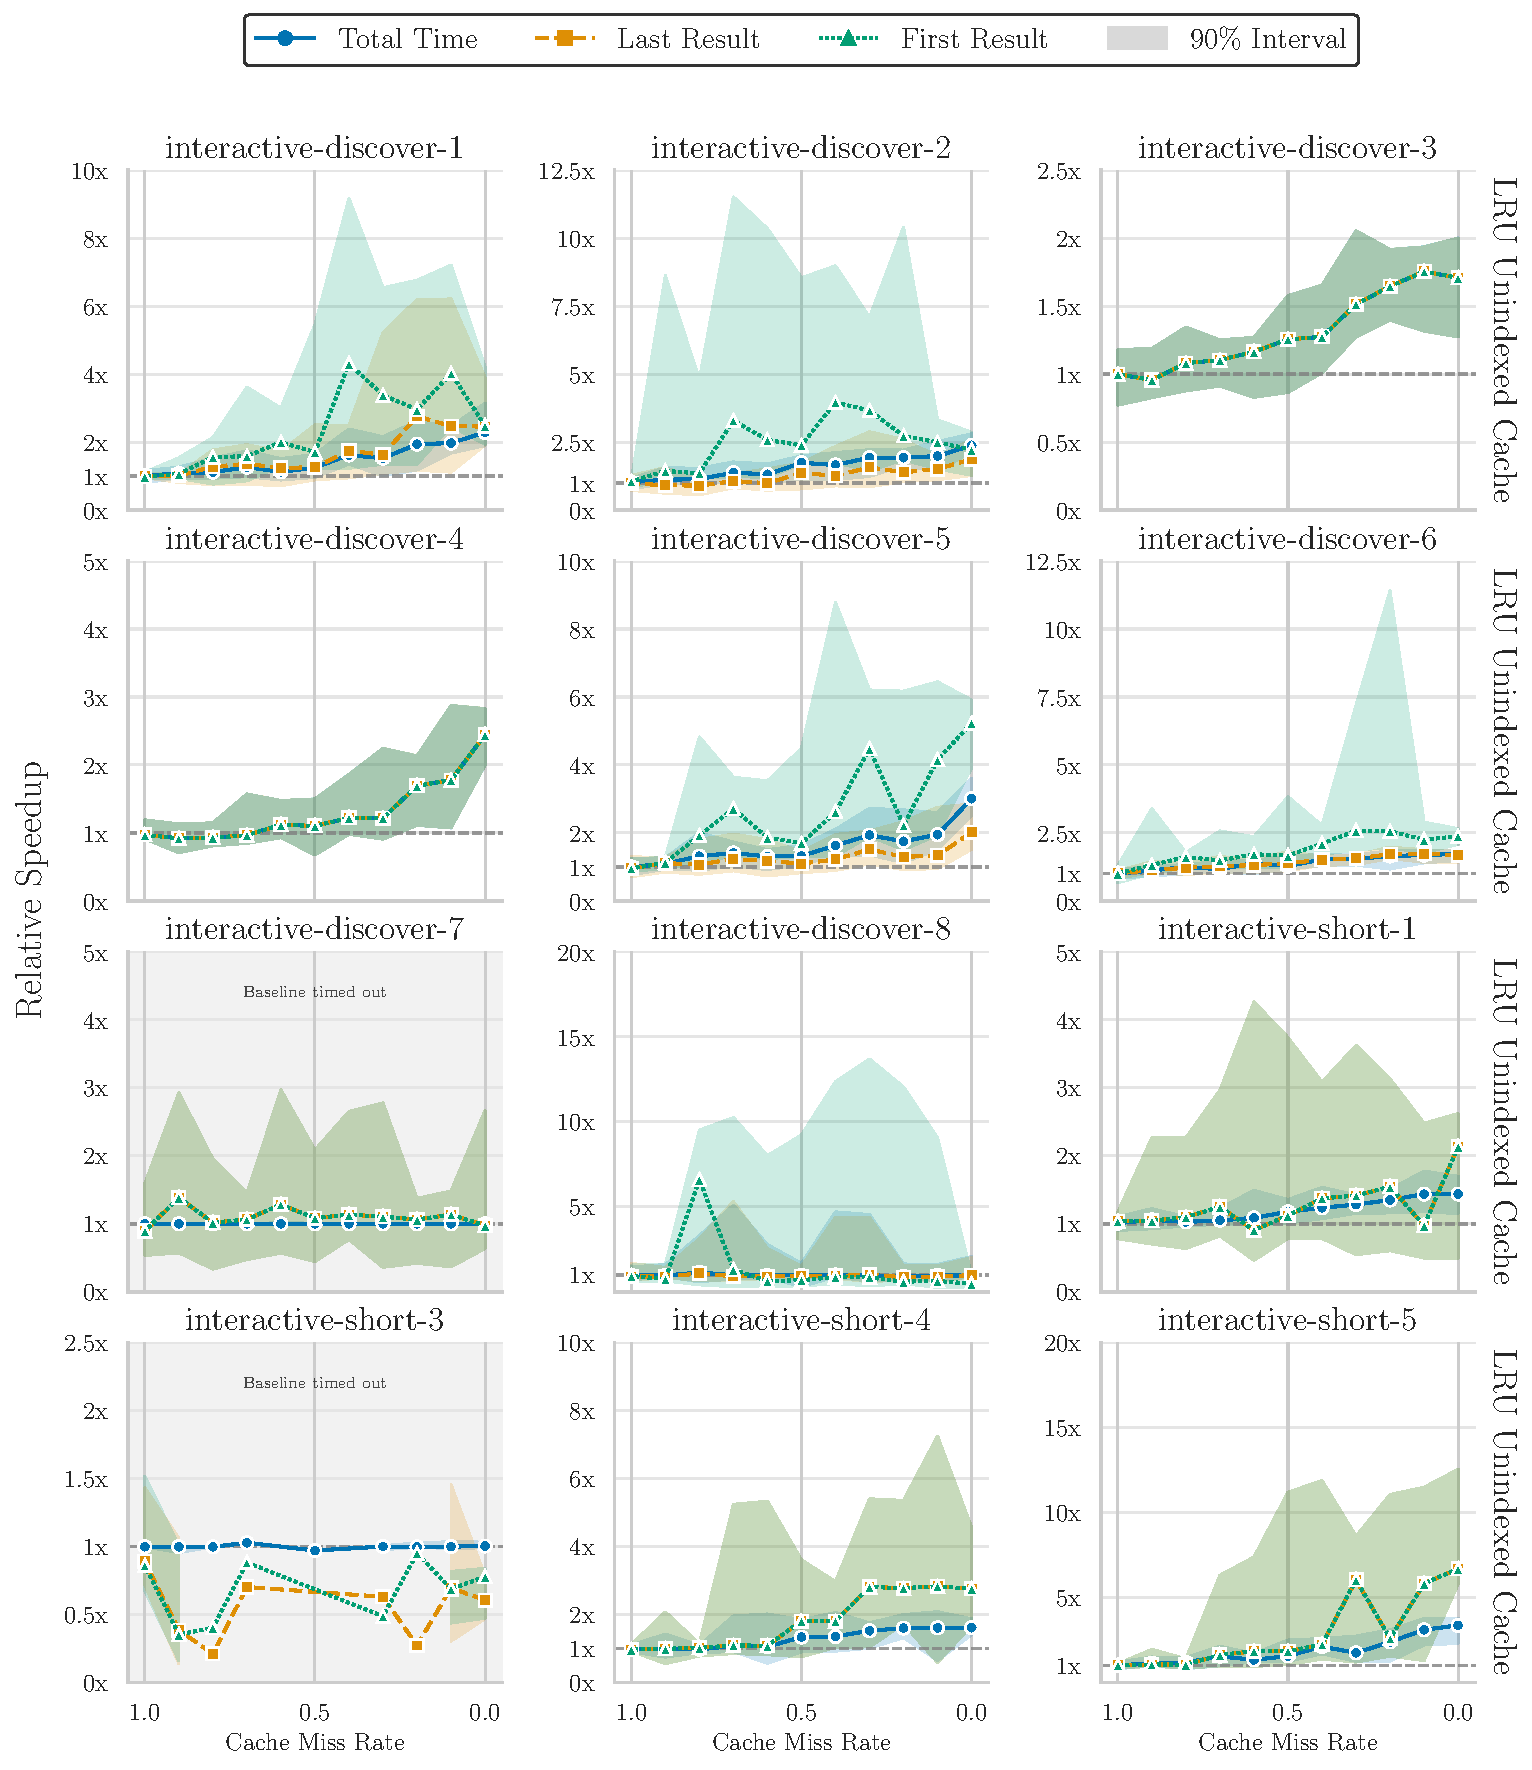
\includegraphics[width=\textwidth]{figures/synth_hit_rate_reduced_lru_unindexed_cache.pdf}
    \caption{ Performance of LRU-based unindexed cache across all query templates. The y-axis shows the mean speedup relative 
    to a baseline with a 0\% hit rate. Shaded regions denote the 90th percentile }
    \label{fig:full-theoretical-unindexed}
\end{figure*}

\begin{figure*}[!h]
    \centering
    % Ensure the filename matches your generated PDF
    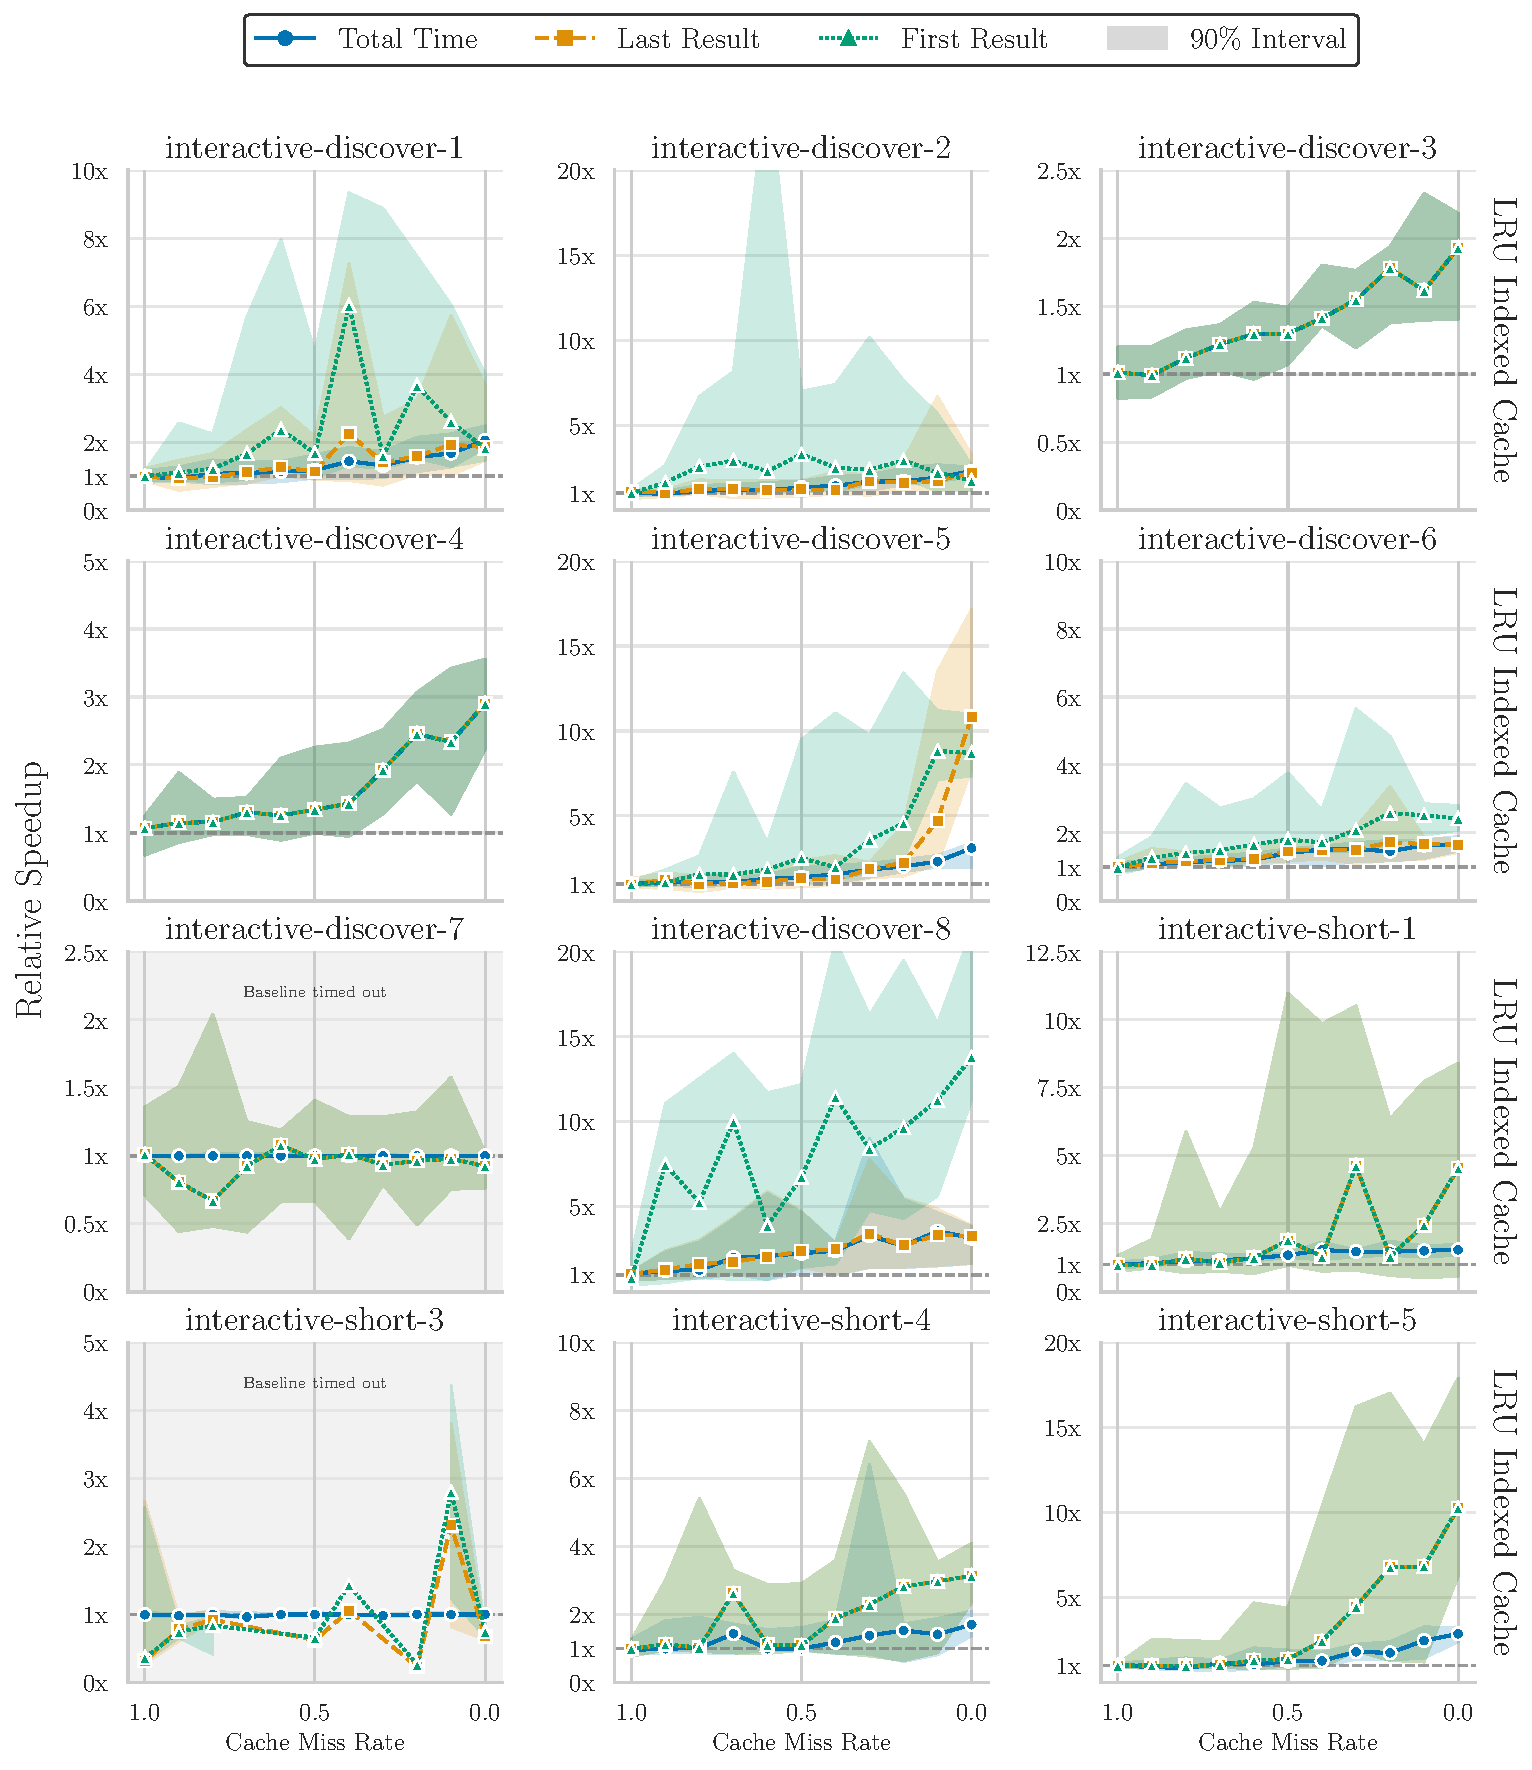
\includegraphics[width=\textwidth]{figures/synth_hit_rate_reduced_lru_indexed_cache.pdf}
    \caption{ Performance of LRU-based indexed cache across all query templates. The y-axis shows the mean speedup relative 
    to a baseline with a 0\% hit rate. Shaded regions denote the 90th percentile }
    \label{fig:full-theoretical-indexed}
\end{figure*}

\begin{figure*}[!h]
    \centering
    % Ensure the filename matches your generated PDF
    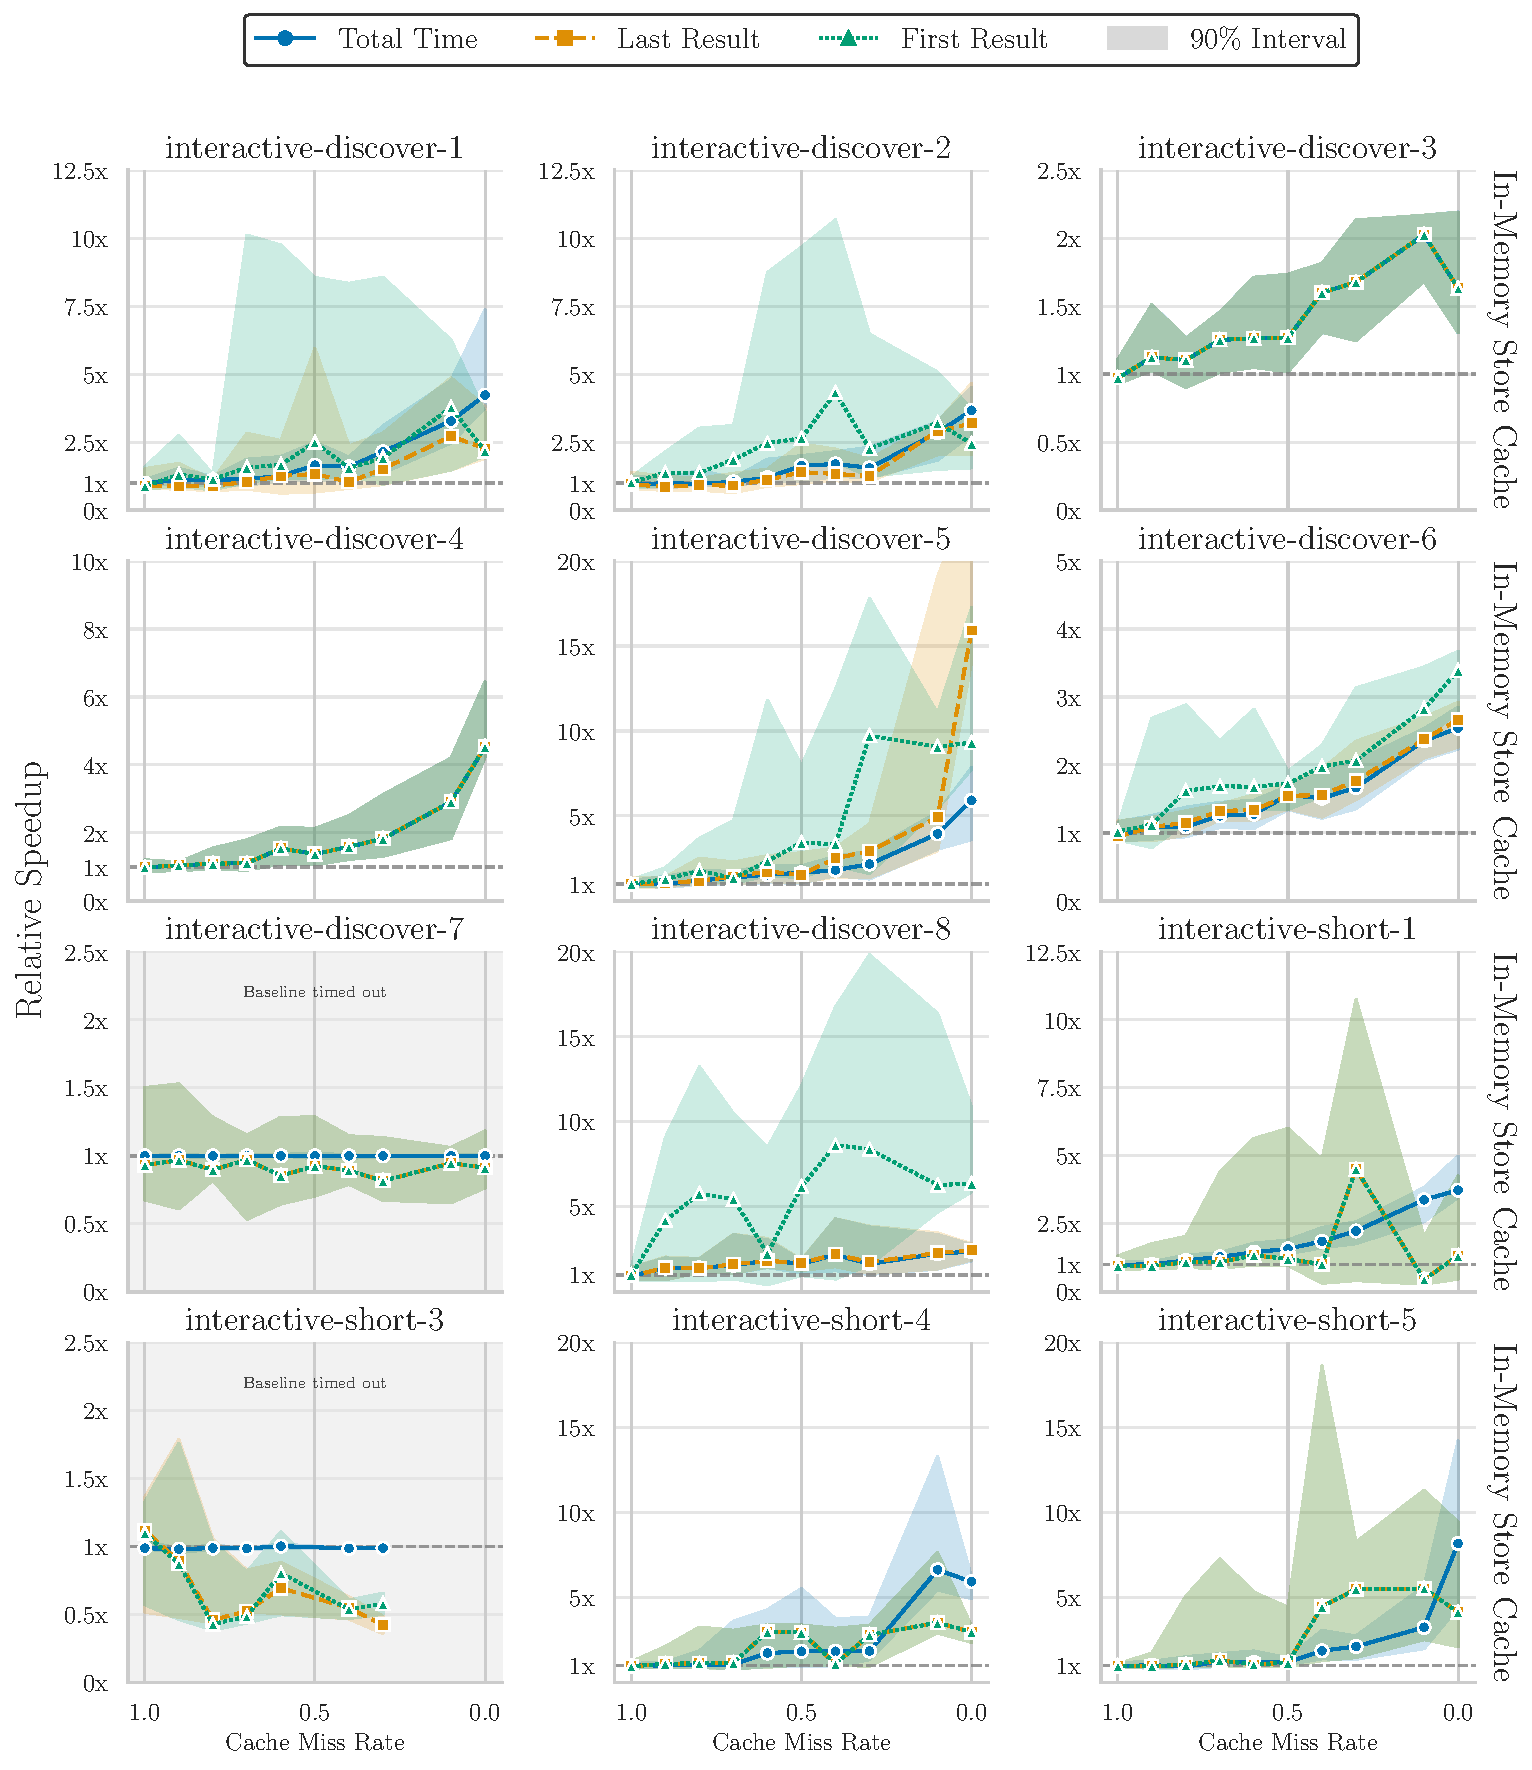
\includegraphics[width=\textwidth]{figures/synth_hit_rate_reduced_in-memory_store_cache.pdf}
    \caption{ Performance of in-memory store cache across all query templates. The y-axis shows the mean speedup relative 
    to a baseline with a 0\% hit rate. Shaded regions denote the 90th percentile }
    \label{fig:full-theoretical-store}
\end{figure*}

\begin{figure*}[!h]
    \centering
    % Ensure the filename matches your generated PDF
    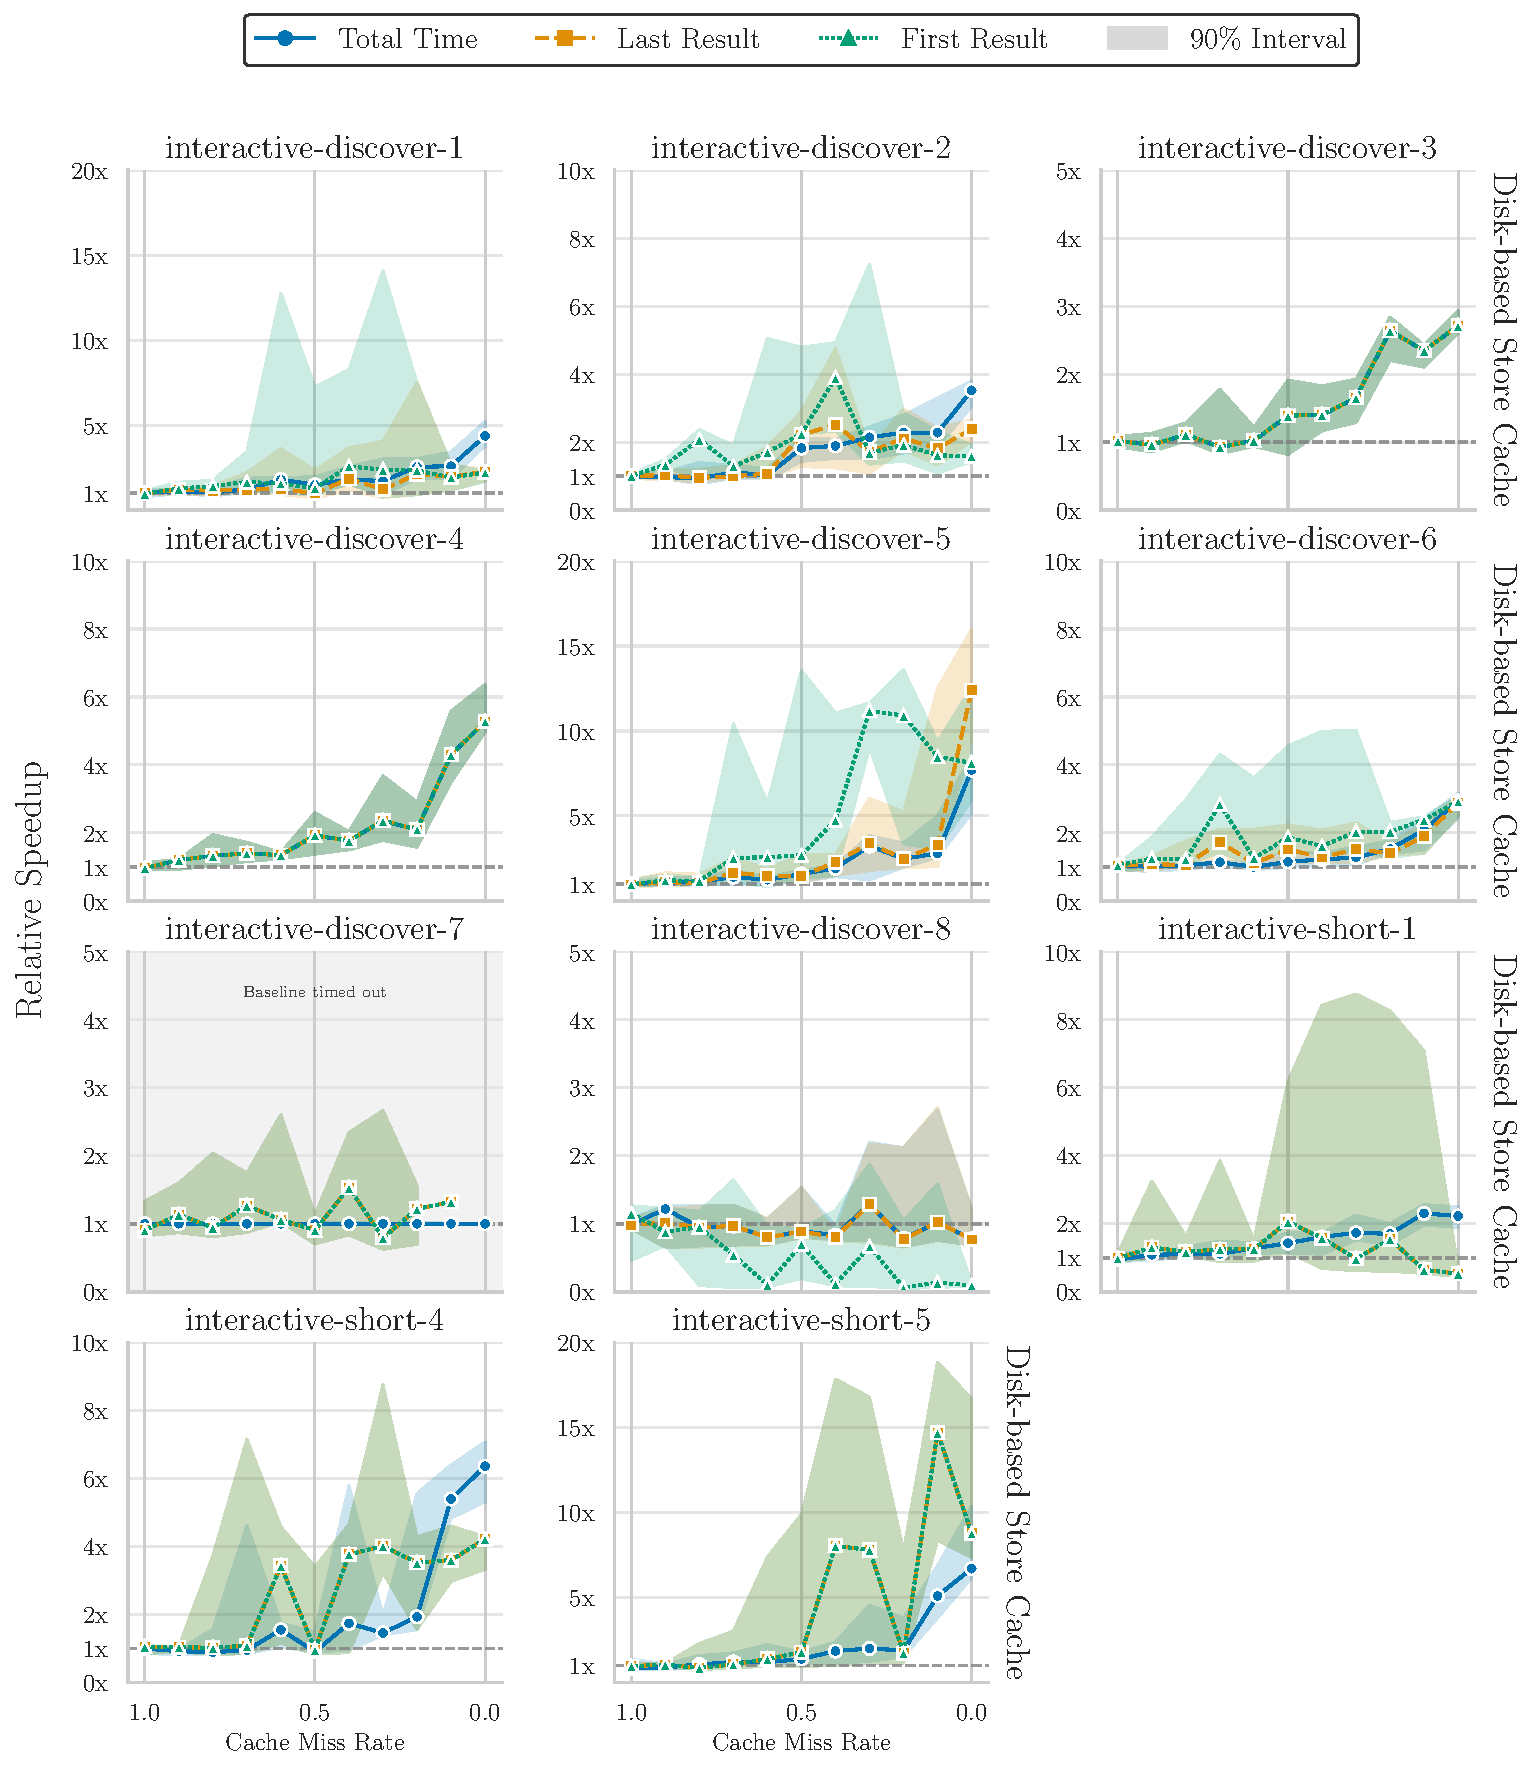
\includegraphics[width=\textwidth]{figures/synth_hit_rate_reduced_disk-based_store_cache.pdf}
    \caption{ Performance of disk-based store cache across all query templates. The y-axis shows the mean speedup relative 
    to a baseline with a 0\% hit rate. Shaded regions denote the 90th percentile }
    \label{fig:full-theoretical-disk}
\end{figure*}
